%  LaTeX support: latex@mdpi.com 
%  For support, please attach all files needed for compiling as well as the log file, and specify your operating system, LaTeX version, and LaTeX editor.

%=================================================================
% UNCOMMENT THE FOLLOWING LINE FOR PRODUCTION WITH mdpi.cls:
\documentclass[journal,article,submit,pdftex,moreauthors]{Definitions/mdpi} 

%=================================================================
% MDPI internal commands
\firstpage{1} 
\makeatletter 
\setcounter{page}{\@firstpage} 
\makeatother
\pubvolume{1}
\issuenum{1}
\articlenumber{0}
\pubyear{2025}
\copyrightyear{2025}
\datereceived{ } 
\daterevised{ } 
\dateaccepted{ } 
\datepublished{ } 
\hreflink{https://doi.org/} 

%=================================================================
% Add packages and commands here.
\usepackage{amsmath}
\usepackage{amssymb}
\usepackage{booktabs} 
\usepackage{multirow}
\usepackage{graphicx}
\usepackage{algorithm}
\usepackage{algorithmic}
\usepackage{bm} 
\usepackage{url}
\usepackage{float}

%=================================================================
% Full title of the paper (Capitalized)
\Title{Adaptive Ensemble Weight Optimization for Natural Gas Consumption Forecasting: A Hybrid Stochastic-Deep Learning Framework Applied to the Czech Market}

% Authors
\Author{Josef Jablonsky $^{1}$ and Vojtěch Vávra $^{1}$*}

% Affiliations
\address{%
$^{1}$ \quad Department of Econometrics, University of Economics and Business, Prague, Czech Republic}

% Contact information
\corres{Correspondence: jablon@vse.cz}

% Abstract
\abstract{The transition towards data-driven energy management necessitates advanced predictive frameworks capable of handling the non-linear and non-stationary nature of natural gas consumption. This study addresses the challenge of creating a robust meta-learner for daily gas consumption forecasting in the Czech Republic by proposing a \textbf{convex ensemble weight optimization} framework. Moving beyond simple model averaging, we formulate the ensemble weighting problem as a constrained convex optimization task on a unit simplex. We propose and evaluate a rigorous methodology utilizing the Frank-Wolfe algorithm (Conditional Gradient) and Ensemble Selection to dynamically optimize weights of a heterogeneous set of base learners, including SARIMAX, XGBoost, N-HiTS, and Temporal Fusion Transformers (TFT). The study is supported by a comprehensive feature engineering pipeline utilizing regulatory data from the Market Operator (OTE). Our results demonstrate that mathematically rigorous weight optimization (MAPE \textbf{4.25\%}) significantly outperforms both individual state-of-the-art models (N-HiTS 5.31\%) and static averaging (6.74\%), offering a direct operational advantage for balancing market participation. We specifically validate a "Recency-Weighted" heuristic, demonstrating its robustness compared to standard exponential decay schemes.}

% Keywords
\keyword{Natural Gas Forecasting; Operations Research; Convex Optimization; Frank-Wolfe Algorithm; Ensemble Learning; Deep Learning; Czech Energy Market} 

%%%%%%%%%%%%%%%%%%%%%%%%%%%%%%%%%%%%%%%%%%
\begin{document}

%%%%%%%%%%%%%%%%%%%%%%%%%%%%%%%%%%%%%%%%%%
\section{Introduction}

The accurate forecasting of natural gas consumption is a cornerstone of energy security and economic efficiency, particularly in countries with high import dependence and seasonal demand variability like the Czech Republic. While individual machine learning (ML) architectures—ranging from Gradient Boosting Machines (GBM) \citep{ref_xgboost} to Recurrent Neural Networks (RNN)—have shown promise, single-model approaches often lack robustness against regime shifts, such as sudden weather anomalies or geopolitical shocks.

This paper shifts the research focus from the development of individual predictors to the \textit{operational research} problem of optimal forecast combination. We hypothesize that the daily prediction task can be modeled as a decision-making process where a meta-learner assigns weights to a portfolio of diverse algorithms.

The contribution of this study is threefold:
\begin{enumerate}
    \item \textbf{Mathematical Formulation:} We frame the ensemble weighting problem as a constrained convex optimization task on a simplex, minimizing a regularized loss function that reflects the asymmetry of balancing costs \citep{ref_boyd}.
    \item \textbf{Algorithmic Solution:} We apply the Frank-Wolfe algorithm \citep{ref_fw_jaggi} and Ensemble Selection methods \citep{ref_caruana} to solve this optimization problem efficiently in a rolling-window production environment.
    \item \textbf{Empirical Validation:} We provide a comprehensive validation on real-world Czech gas consumption data, explicitly comparing our "Recency-Weighted" heuristic against standard exponential decay and identifying the optimal memory length.
\end{enumerate}

%%%%%%%%%%%%%%%%%%%%%%%%%%%%%%%%%%%%%%%%%%
\section{Literature Review}

The forecasting of energy consumption has undergone a paradigm shift from traditional econometric approaches to advanced artificial intelligence methods. This section reviews the evolution of these methodologies with a focus on their application to natural gas markets.

\subsection{Statistical and Machine Learning Approaches}
Historically, statistical linear models such as ARIMA (AutoRegressive Integrated Moving Average) and its seasonal variants (SARIMAX) were the industry standard. However, forecasting natural gas consumption involves capturing complex non-linear dependencies on meteorological factors, which linear models often fail to address adequately. As noted by \citep{ref_mdpi_energies_1}, methods like Multivariate Adaptive Regression Splines (MARS) have been proposed to handle these non-linearities better than traditional regression.
Subsequently, machine learning algorithms such as Support Vector Regression (SVR) and Random Forests gained prominence. \citep{Dudek2021} demonstrated the effectiveness of Random Forest for short-term load forecasting across multiple datasets, highlighting its robustness to non-stationarity and multiple seasonal cycles. These ``shallow'' learning methods remain relevant due to their interpretability and lower computational costs compared to deep neural networks.


\subsection{Deep Learning and Transformer Models}
In recent years, Deep Learning has achieved state-of-the-art results in time series forecasting. Long Short-Term Memory (LSTM) networks are widely used to model temporal sequences, as demonstrated by \citep{ref_mdpi_math_1} in the context of long-term energy consumption. 
More recently, Transformer-based architectures have revolutionized the field. The \textbf{Temporal Fusion Transformer (TFT)} \citep{ref_tft} introduces a multi-head attention mechanism combined with variable selection networks, offering both high accuracy and interpretability regarding feature importance. Another significant development is \textbf{N-HiTS} (Neural Hierarchical Interpolation for Time Series) \citep{ref_nhits}, which reduces the computational complexity of Transformers by using hierarchical blocks to capture different frequency components of the signal.

\subsection{Ensemble Learning Taxonomy and Positioning}
Ensemble methods for time series forecasting can be broadly categorized into three groups, as synthesized by \citep{ref_wu_review} and \citep{ref_oliveira}:
\begin{enumerate}
    \item \textbf{Bagging and Boosting:} Techniques like Random Forests or XGBoost generate diversity by training models on different subsets of data or by iteratively correcting errors. These are method-centric approaches aimed at reducing variance or bias of a specific learner.
    \item \textbf{Meta-Learning / Stacking:} A secondary "meta-model" learns to combine the predictions of base learners, often using complex non-linear functions. While powerful, these can be prone to overfitting if data is limited.
    \item \textbf{Convex Weight Optimization:} This approach, which we adopt, seeks an optimal linear combination of pre-trained heterogeneous models. Unlike black-box meta-learners, it imposes constraints (e.g., weights sum to one, non-negativity) that provide interpretability similar to a financial portfolio.
\end{enumerate}

Despite the efficacy of individual models, the "No Free Lunch" theorem suggests that no single model performs best under all conditions. \citep{ref_mdpi_energies_2} highlight that dynamic ensemble strategies can effectively mitigate the bias-variance trade-off and adapt to changing market regimes. Our work contributes to the third category (Convex Weight Optimization) by applying the Frank-Wolfe algorithm to dynamically optimize ensemble weights on the unit simplex. This ensures a robust and mathematically grounded combination strategy that is distinct from simple averaging or heuristic selection.

%%%%%%%%%%%%%%%%%%%%%%%%%%%%%%%%%%%%%%%%%%
\section{Materials and Methods}

We propose a \textbf{Three-Layer Ensemble Framework} for robust forecasting:
\begin{enumerate}
    \item \textbf{Layer 1: Base Learners:} A diverse library of 15 heterogeneous algorithms generating independent forecasts.
    \item \textbf{Layer 2: Temporal Weighting Strategy:} A mechanism to define the importance of historical data (e.g., Recency-Weighted) to handle regime shifts.
    \item \textbf{Layer 3: Ensemble Optimizer:} A convex solver (Frank-Wolfe) that computes the optimal weights $\mathbf{w}$ based on the weighted history.
\end{enumerate}

The methodology is implemented in Python 3.11, utilizing libraries such as \texttt{pandas} for data manipulation, \texttt{pytorch} \citep{ref_pytorch} for deep learning models, and custom solvers for optimization tasks.

\subsection{Data Engineering and Feature Selection}
The primary dataset consists of daily gas consumption series in the Czech Republic, sourced from the Market Operator (OTE, a.s.) \citep{ref_ote}. Weather data (temperature, wind speed) were obtained via the Open-Meteo API \citep{ref_openmeteo}, utilizing the ERA5 reanalysis model for historical data. To ensure spatial representativeness for the entire Czech Republic, we aggregated data from the geographic centroids of all administrative districts (okresy). The daily values were resampled to align with the "Gas Day" convention (06:00 AM to 06:00 AM next day).

A critical preprocessing step, mandated by the regulatory framework, is the calculation of Effective Temperature ($T_{eff}$). Unlike raw air temperature, $T_{eff}$ accounts for the thermal inertia of buildings. We implement the recursive filter defined by OTE:
\begin{equation}
    T_{eff, t} = 0.5 \cdot T_t + 0.5 \cdot T_{eff, t-1}
\end{equation}
Additional engineered features include:
\begin{itemize}
    \item \textbf{Calendar Features:} Boolean flags for weekends and public holidays (using the \texttt{holidays} library for CZ), and cyclical encodings ($\sin \frac{2\pi d}{365}, \cos \frac{2\pi d}{365}$) of the day of year.
    \item \textbf{Lagged Variables:} Consumption lags ($t-1, t-2, t-7, t-14$) to capture short-term and weekly autoregressive properties.
    \item \textbf{Rolling Statistics:} 3-day and 7-day moving averages of temperature and wind speed to smooth out weather volatility.
\end{itemize}

As shown in Figure \ref{fig:feature_importance}, Ridge Regression coefficients confirm that effective temperature and immediate consumption history are the most significant linear predictors. The negative coefficient for temperature confirms the inverse relationship with heating demand.

\begin{figure}[H]
\centering
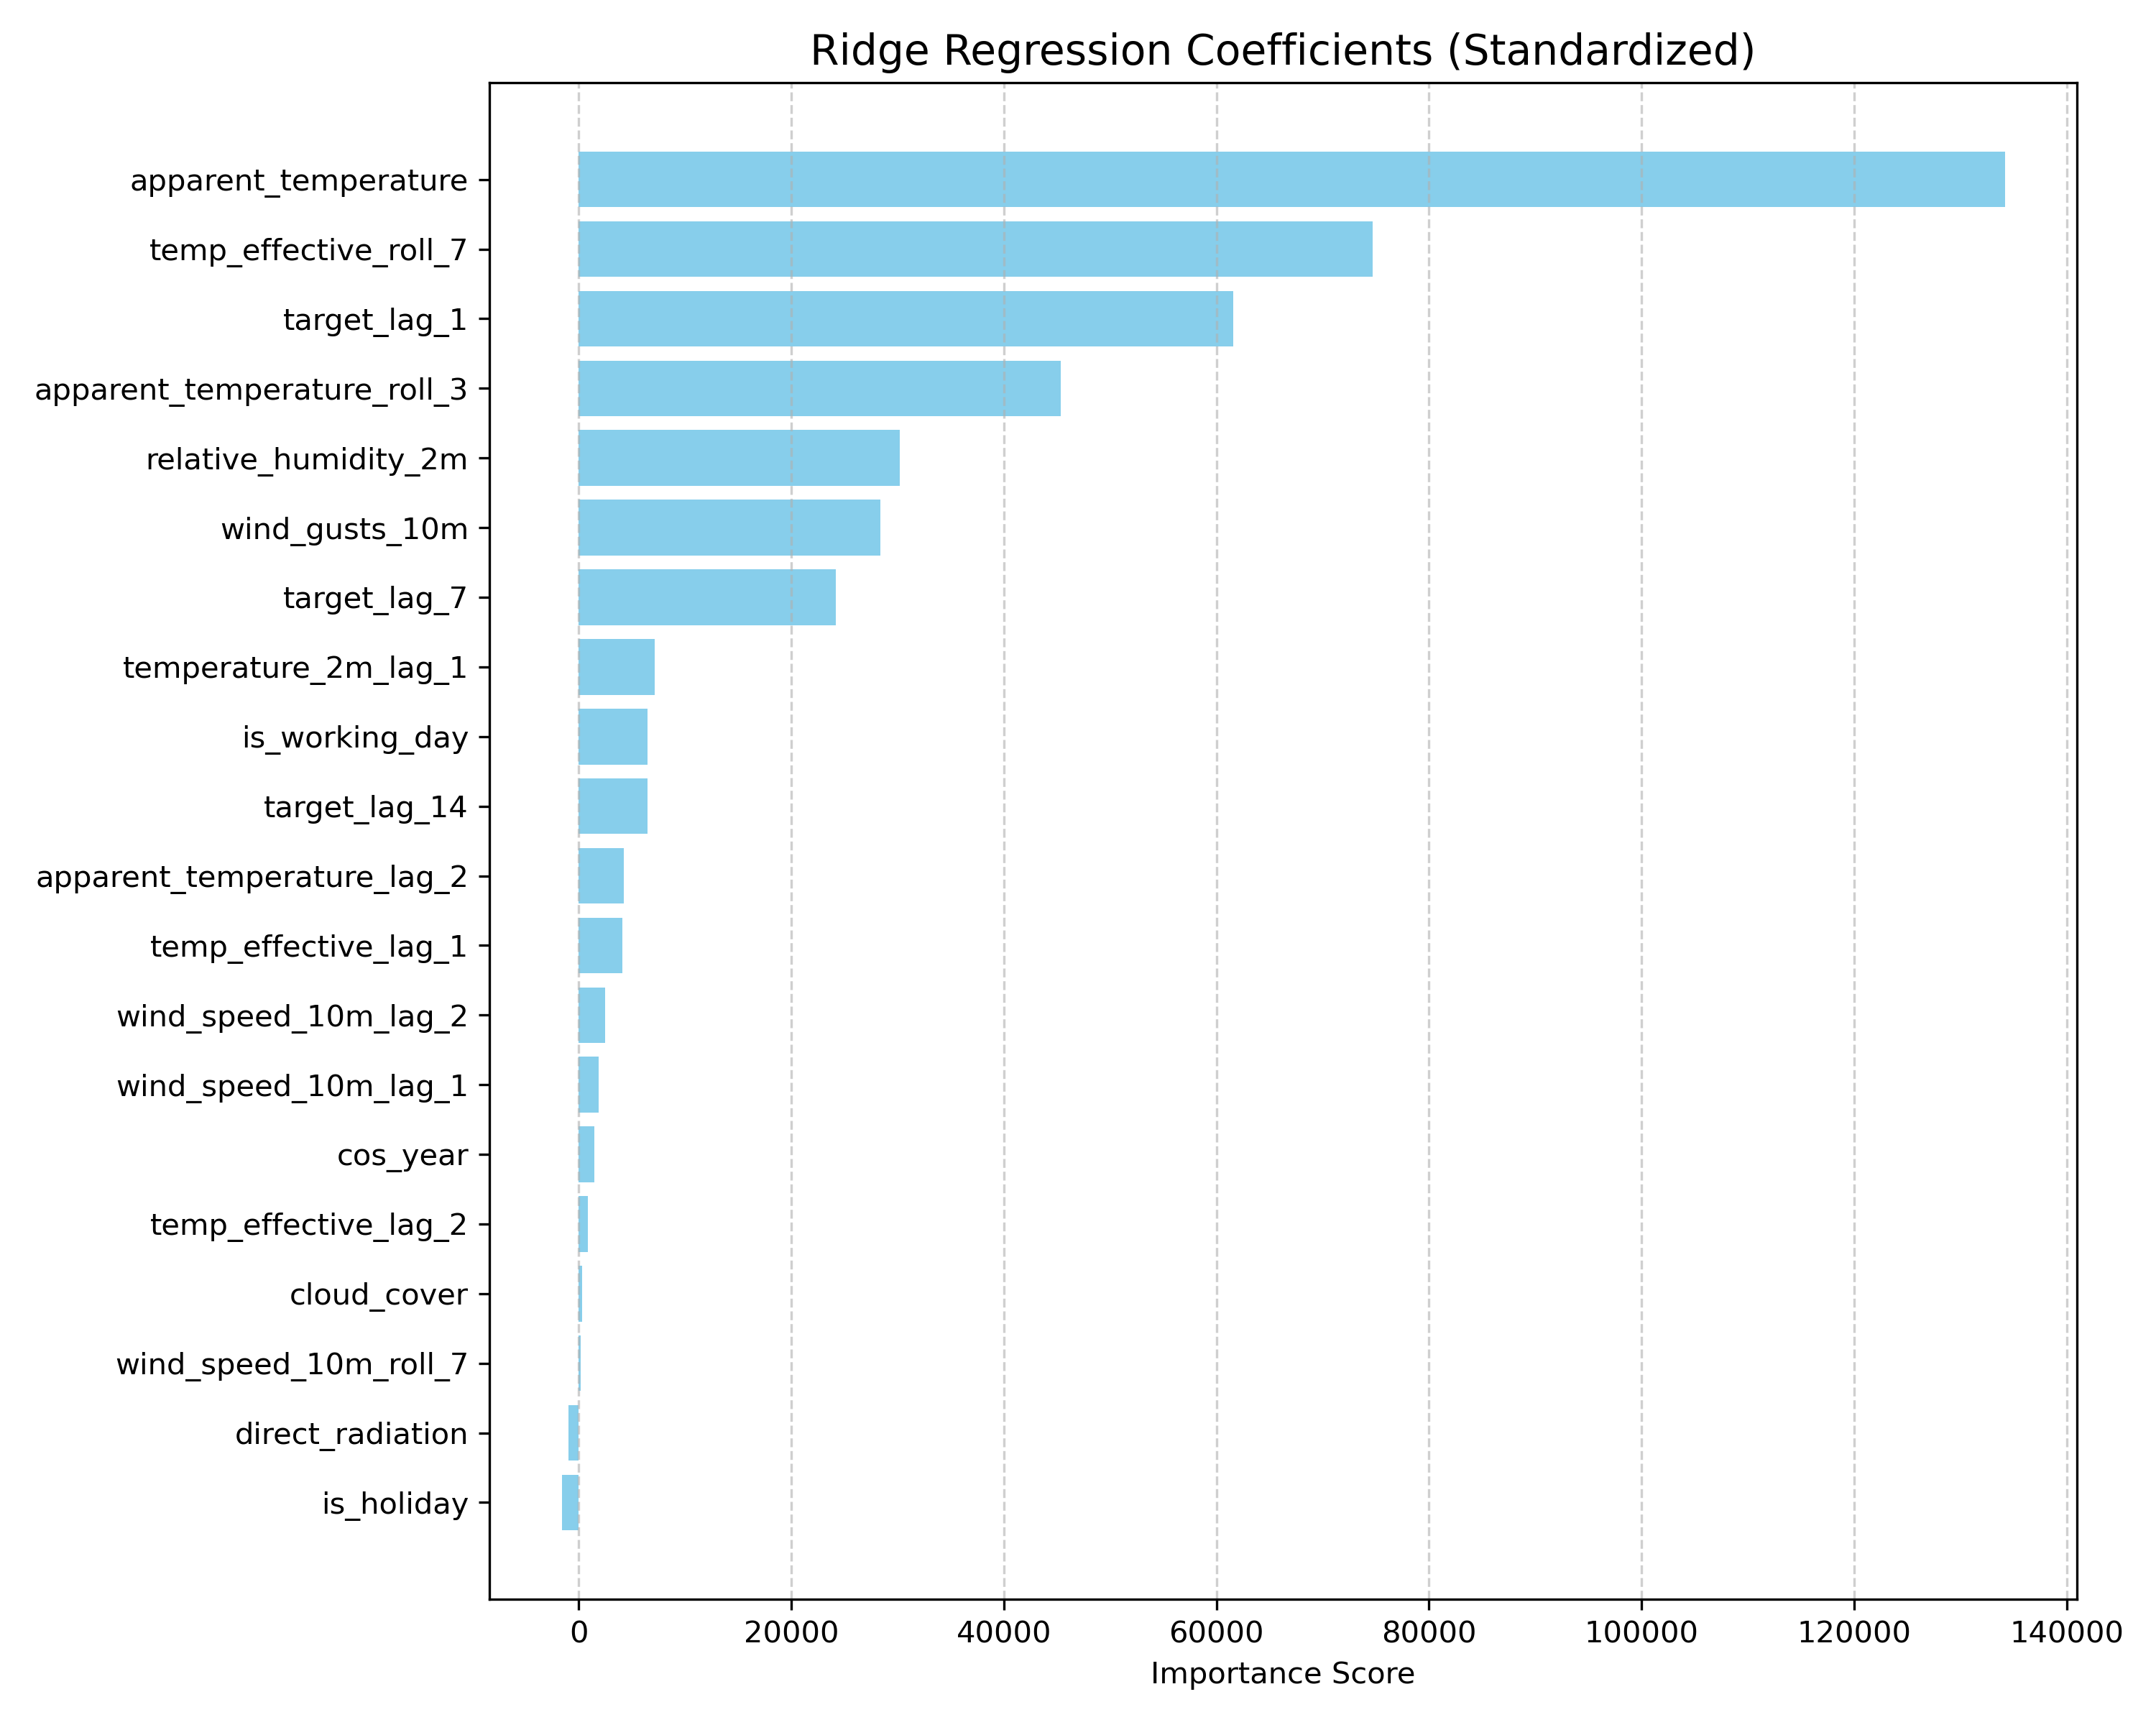
\includegraphics[width=0.8\textwidth]{feature_importance_ridge.png}
\caption{Feature Importance derived from Ridge Regression coefficients. The magnitude indicates the strength of the linear relationship. Effective temperature (negative coefficient) and recent consumption lags (positive coefficients) are the dominant drivers.}
\label{fig:feature_importance}
\end{figure}

\subsection{Base Learners (The Ensemble)}
We employ a heterogeneous set of 15 algorithms to ensure error independence and diversity.

\subsubsection{Tree-Based Ensembles}
We utilized \textbf{XGBoost} \citep{ref_xgboost}, \textbf{LightGBM} \citep{ref_lgbm}, \textbf{CatBoost} \citep{ref_catboost}, and \textbf{ExtraTrees} \citep{ref_scikit}. These models are robust to outliers and capable of modeling non-linear interactions. Hyperparameters were tuned using the Tree-structured Parzen Estimator (TPE) algorithm.

\subsubsection{Deep Learning Architectures}
\begin{itemize}
    \item \textbf{LSTM (Long Short-Term Memory):} Recurrent networks designed to capture temporal dependencies \citep{ref_pytorch}.
    \item \textbf{TFT (Temporal Fusion Transformer):} An attention-based architecture proposed by \citep{ref_tft} that provides interpretability and explicitly handles static (location) and dynamic (time) covariates.
    \item \textbf{N-HiTS (Neural Hierarchical Interpolation for Time Series):} A state-of-the-art model by \citep{ref_nhits} using hierarchical interpolation for long-range dependencies.
    \item \textbf{NeuralProphet:} A hybrid model bridging statistical and deep learning approaches, based on PyTorch \citep{ref_pytorch}.
\end{itemize}

Deep learning models (TFT, N-HiTS) were tuned using a grid search over learning rate and dropout focusing on the validation set performance to ensure stability.

\subsubsection{Statistical and Econometric Models}
To provide a robust baseline, we included \textbf{SARIMAX} (Seasonal AutoRegressive Integrated Moving Average with eXogenous factors) and \textbf{Prophet} \citep{ref_prophet}. Additionally, a robust \textbf{ARX} model (AutoRegression with Exogenous variables) was implemented using the SARIMAX backend to handle structural breaks.

\subsubsection{Classical Machine Learning}
We further diversified the pool with classical algorithms implemented via Scikit-learn \citep{ref_scikit}:
\begin{itemize}
    \item \textbf{SVR (Support Vector Regression):} Effective in high-dimensional spaces.
    \item \textbf{ElasticNet:} A regularized regression method combining L1 and L2 penalties.
    \item \textbf{Bayesian Ridge:} Probabilistic approach to linear regression.
    \item \textbf{KNN (K-Nearest Neighbors):} A non-parametric method based on feature similarity.
\end{itemize}

\subsection{Optimization Framework: The Frank-Wolfe Algorithm}
The core technical innovation is the dynamic weighting mechanism. Let $\hat{y}_{i,t}$ be the prediction of model $i$ at time $t$, and $y_t$ be the actual consumption. We seek a weight vector $\mathbf{w} \in \mathbb{R}^N$ that minimizes the loss function $\mathcal{L}$ over a historical window $H$.

The optimization problem is defined as:
\begin{align}
    \min_{\mathbf{w}} \quad & f(\mathbf{w}) = \frac{1}{H} \sum_{t=1}^H \mathcal{L}\left(y_t, \sum_{i=1}^N w_i \hat{y}_{i,t}\right) \\
    \text{s.t.} \quad & \sum_{i=1}^N w_i = 1, \quad w_i \ge 0 \quad (\mathbf{w} \in \Delta_N)
\end{align}

To solve this, we utilize the Frank-Wolfe algorithm (Algorithm \ref{alg:fw}), originally proposed by \citep{ref_fw_orig}, which avoids computationally expensive projections onto the simplex. A key computational advantage over Projected Gradient Descent is that the Linear Minimization Oracle (LMO) naturally returns a vertex of the simplex, eliminating the need for computationally expensive projection steps.

\textbf{Theoretical Note on Convexity:} In practical implementation, weights are optimized using either MSE or MAPE. The theoretical discussion regarding convergence guarantees strictly applies to the MSE (convex case), whereas the application to MAPE is validated empirically. Note that for MAPE, differentiability issues at zero are theoretically possible but practically irrelevant for gas consumption data (which is strictly positive). Furthermore, the limited number of iterations $K$ (set to 500) provides an \textbf{implicit regularization}, producing sparse solutions akin to early stopping in gradient methods \citep{ref_fw_jaggi}.

\begin{algorithm}[H]
\caption{Frank-Wolfe for Ensemble Weights Optimization}
\label{alg:fw}
\begin{algorithmic}[1]
\STATE \textbf{Input:} Initial weights $\mathbf{w}^{(0)} \in \Delta_N$, tolerance $\epsilon$
\FOR{$k = 0 \dots K$}
    \STATE Compute gradient $\nabla f(\mathbf{w}^{(k)})$
    \STATE \textit{Linear Minimization Oracle (LMO):}
    \STATE $\mathbf{s}^{(k)} \leftarrow \arg\min_{\mathbf{s} \in \Delta_N} \langle \mathbf{s}, \nabla f(\mathbf{w}^{(k)}) \rangle$
    \STATE \textit{For a linear function on a simplex, the solution to the LMO is the vertex (representing a single model) corresponding to the component with the largest negative gradient (or smallest gradient value). This property renders the step computationally inexpensive compared to projection methods.}
    \STATE Calculate step size $\gamma \leftarrow \frac{2}{k+2}$
    \STATE Update: $\mathbf{w}^{(k+1)} \leftarrow (1-\gamma)\mathbf{w}^{(k)} + \gamma \mathbf{s}^{(k)}$
\ENDFOR
\STATE \textbf{Output:} Optimized weights $\mathbf{w}^{(K)}$
\end{algorithmic}
\end{algorithm}

\subsection{Benchmark Ensemble Strategies}
To rigorously evaluate the performance of the Frank-Wolfe optimization, we compare it against several established ensemble techniques:

\begin{itemize}
    \item \textbf{Ensemble Selection} \citep{ref_caruana}: This is a "greedy" optimization algorithm. Instead of analytically solving a complex equation, it iteratively constructs the ensemble. Starting with an empty set, in each iteration, it adds the single model from the pool that maximizes the performance (minimizes MSE) of the current ensemble.
    \item \textbf{NNLS (Non-Negative Least Squares):} This method solves the standard least squares problem subject to the constraint $w_i \ge 0$. In the context of energy consumption forecasting, negative weights are physically uninterpretable.
    \item \textbf{Contextual Bandits (LinUCB):} We frame the model selection as a problem from the domain of Reinforcement Learning. An "agent" observes the current context (weather, day of week, season) and decides which model to trust.
    \item \textbf{Simple Ensemble Average:} This serves as the baseline benchmark ($w_i = 1/15$).
\end{itemize}

\subsection{Historical Data Weighting Schemes}
To enhance the model's adaptability to sudden trend changes (e.g., rapid temperature drops), we incorporate a weighting mechanism into the loss function. The objective is to minimize a \textbf{weighted sum of errors} over the historical window $H$.

Formally, we define the weighted loss function as:
\begin{equation}
    \min_{\mathbf{w} \in \Delta_N} \sum_{t=1}^H \omega_t \cdot \mathcal{L}\left(y_t, \sum_{i=1}^N w_i \hat{y}_{i,t}\right)
\end{equation}
where $\omega_t$ represents the importance of observation $t$. It is worth noting that a non-negative linear combination of convex functions remains convex, ensuring that the introduction of weights $\omega_t$ preserves the convergence properties of the Frank-Wolfe algorithm for convex base losses (e.g., MSE). We evaluate three distinct strategies:

\begin{enumerate}
    \item \textbf{Standard (Rolling Window):} All observations $t$ in the history window $H$ have equal weight $\omega_t = 1$.
    \item \textbf{Recency-Weighted Heuristic:} We formally define this method through a \textbf{Weighted Loss Function} where weights $\omega_t$ are adjusted to reflect temporal relevance. Specifically, observations $t \in T_{recent}$ (the most recent week) are assigned a weight $\omega_t = 3$, while older observations retain $\omega_t = 1$. The value $\omega_t = 3$ was selected based on preliminary tuning on the validation set, where it demonstrated a robust trade-off between reactivity to new trends and resistance to noise. While this can be computationally implemented by duplicating rows in the input matrix for efficiency, the mathematical definition relies on the weighted objective function in Equation (4).
    \item \textbf{Exponential Decay:} A continuous decay function where $\omega_t = \alpha^{T-t}$.
\end{enumerate}

%%%%%%%%%%%%%%%%%%%%%%%%%%%%%%%%%%%%%%%%%%
\section{Results}

The proposed methodology was evaluated on an out-of-sample test set spanning a full year to ensure the robustness of results across different seasons.

\subsection{Base Model Performance}
The performance of individual models varied significantly (Table \ref{tab:base_models}). The N-HiTS model emerged as the best single predictor with a Mean Absolute Percentage Error (MAPE) of 5.31\%, closely followed by the Temporal Fusion Transformer (TFT) at 5.43\%. Tree-based models (CatBoost, XGBoost, LightGBM) followed with MAPE around 7.3-7.7\%.

\begin{table}[H]
\caption{Performance of Individual Base Learners (Sorted by MAPE)}
\label{tab:base_models}
\centering
\begin{tabular}{lccc}
\toprule
\textbf{Model} & \textbf{MAE (MWh)} & \textbf{RMSE (MWh)} & \textbf{MAPE (\%)} \\
\midrule
N-HiTS & 10,253 & 13,893 & 5.31 \\
Temporal Fusion Transformer (TFT) & 10,050 & 13,321 & 5.43 \\
CatBoost & 13,798 & 18,447 & 7.37 \\
LightGBM & 13,437 & 17,888 & 7.35 \\
Support Vector Regression (SVR) & 14,726 & 20,483 & 7.74 \\
XGBoost & 14,560 & 19,338 & 7.76 \\
ExtraTrees & 15,117 & 19,453 & 8.32 \\
ARX (Robust) & 14,946 & 18,659 & 9.17 \\
Bayesian Ridge & 14,852 & 18,451 & 9.18 \\
ElasticNet & 17,071 & 20,510 & 10.67 \\
NeuralProphet & 17,963 & 22,245 & 11.74 \\
KNN & 21,115 & 26,519 & 12.37 \\
LSTM & 21,293 & 26,591 & 12.91 \\
SARIMAX & 18,840 & 25,071 & 13.05 \\
Prophet & 19,161 & 24,113 & 13.15 \\
\bottomrule
\end{tabular}
\end{table}

A visual comparison of the predictions from base model groups against the actual consumption is presented in Figure \ref{fig:base_models_grouped}.

\begin{figure}[H]
\centering
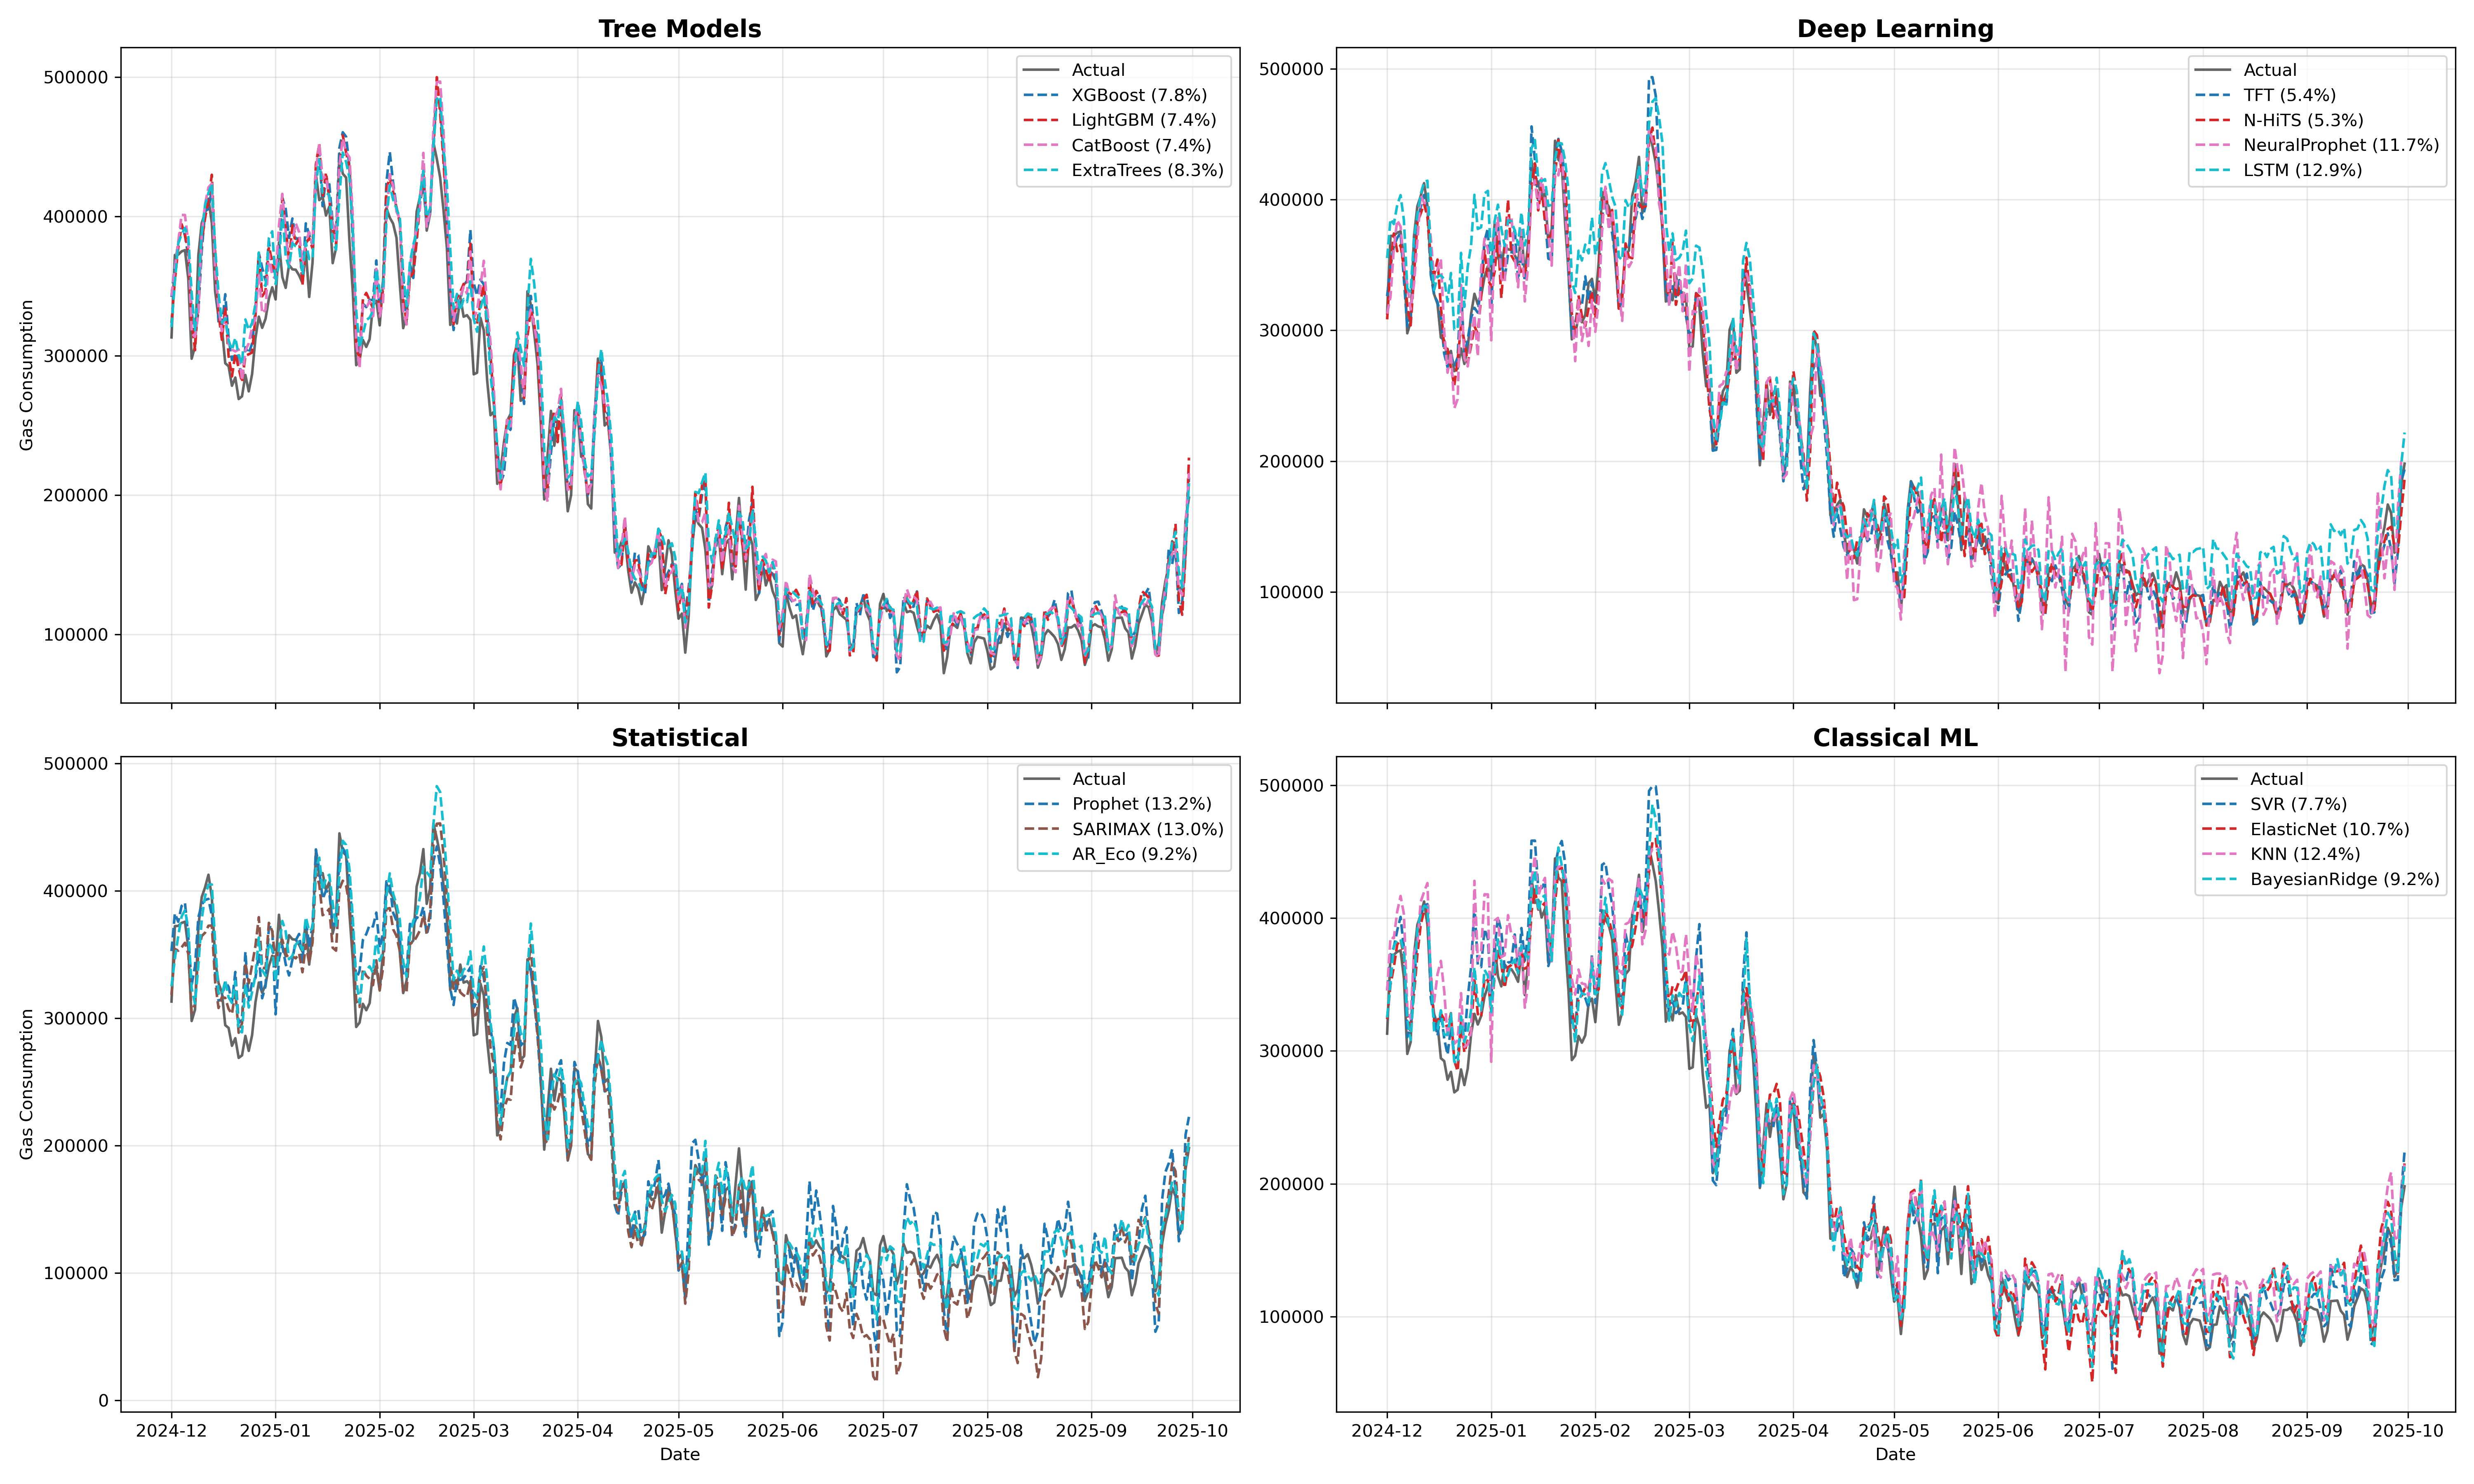
\includegraphics[width=0.95\textwidth]{report_base_models_grouped.png}
\caption{Comparison of base learner predictions grouped by model family (Tree Models, Deep Learning, Statistical, Classical ML) against actual consumption. Deep learning models exhibit the tightest fit to the ground truth.}
\label{fig:base_models_grouped}
\end{figure}

\subsection{Ensemble Optimization Results}
The application of dynamic weighting strategies yielded substantial improvements. Table \ref{tab:ensemble_results} summarizes the performance of different optimization strategies using a 6-week history window, which proved to be optimal in our extended analysis.

\begin{table}[H]
\caption{Comparison of Optimal Ensemble Strategies (6-Week Window)}
\label{tab:ensemble_results}
\centering
\begin{tabular}{lccc}
\toprule
\textbf{Strategy} & \textbf{MAE} & \textbf{RMSE} & \textbf{MAPE (\%)} \\
\midrule
\textbf{Frank-Wolfe (6 weeks, Weighted)} & \textbf{8,235} & \textbf{11,375} & \textbf{4.25} \\
Ensemble Selection (6 weeks, Weighted) & 8,279 & 11,447 & 4.26 \\
Ensemble Selection (6 weeks, Exponential) & 8,202 & 11,260 & 4.26 \\
Frank-Wolfe (6 weeks, Exponential) & 8,221 & 11,345 & 4.27 \\
NNLS (6 weeks, Weighted) & 9,000 & 12,379 & 4.66 \\
\midrule
\textit{Benchmarks:} & & & \\
Best Single Model (N-HiTS) & 10,253 & 13,893 & 5.31 \\
Contextual Bandit (Online) & 10,050 & 13,321 & 5.43 \\
Simple Ensemble Average & 11,723 & 14,897 & 6.74 \\
\bottomrule
\end{tabular}
\end{table}

\begin{enumerate}
    \item \textbf{Superiority of Optimization:} The optimized ensemble achieved a MAPE of \textbf{4.25\%}, reducing the error by more than 1 percentage point relative to the best single model (N-HiTS) and by 2.5 percentage points relative to static averaging.
    \item \textbf{The "Sweet Spot" of Memory:} Our extended analysis identified that a 6-week lookback window provides the optimal balance. Stability increases up to 6 weeks before data drift starts to affect the results. This sensitivity analysis is visualized in Figure \ref{fig:sensitivity}.
    \item \textbf{Validation of "Recency-Weighted" Heuristic:} We explicitly compared our proposed "Recency-Weighted" strategy against a standard exponential decay. The Weighted approach (4.25\%) performed slightly better than Exponential (4.27\%) in the Frank-Wolfe framework, validating the simple heuristic as a robust choice.
    \item \textbf{Method Comparison:} Frank-Wolfe consistently outperformed NNLS (4.66\%). The iterative nature of Frank-Wolfe ($K=500$) acts as an effective regularization against overfitting.
\end{enumerate}

\begin{figure}[H]
\centering
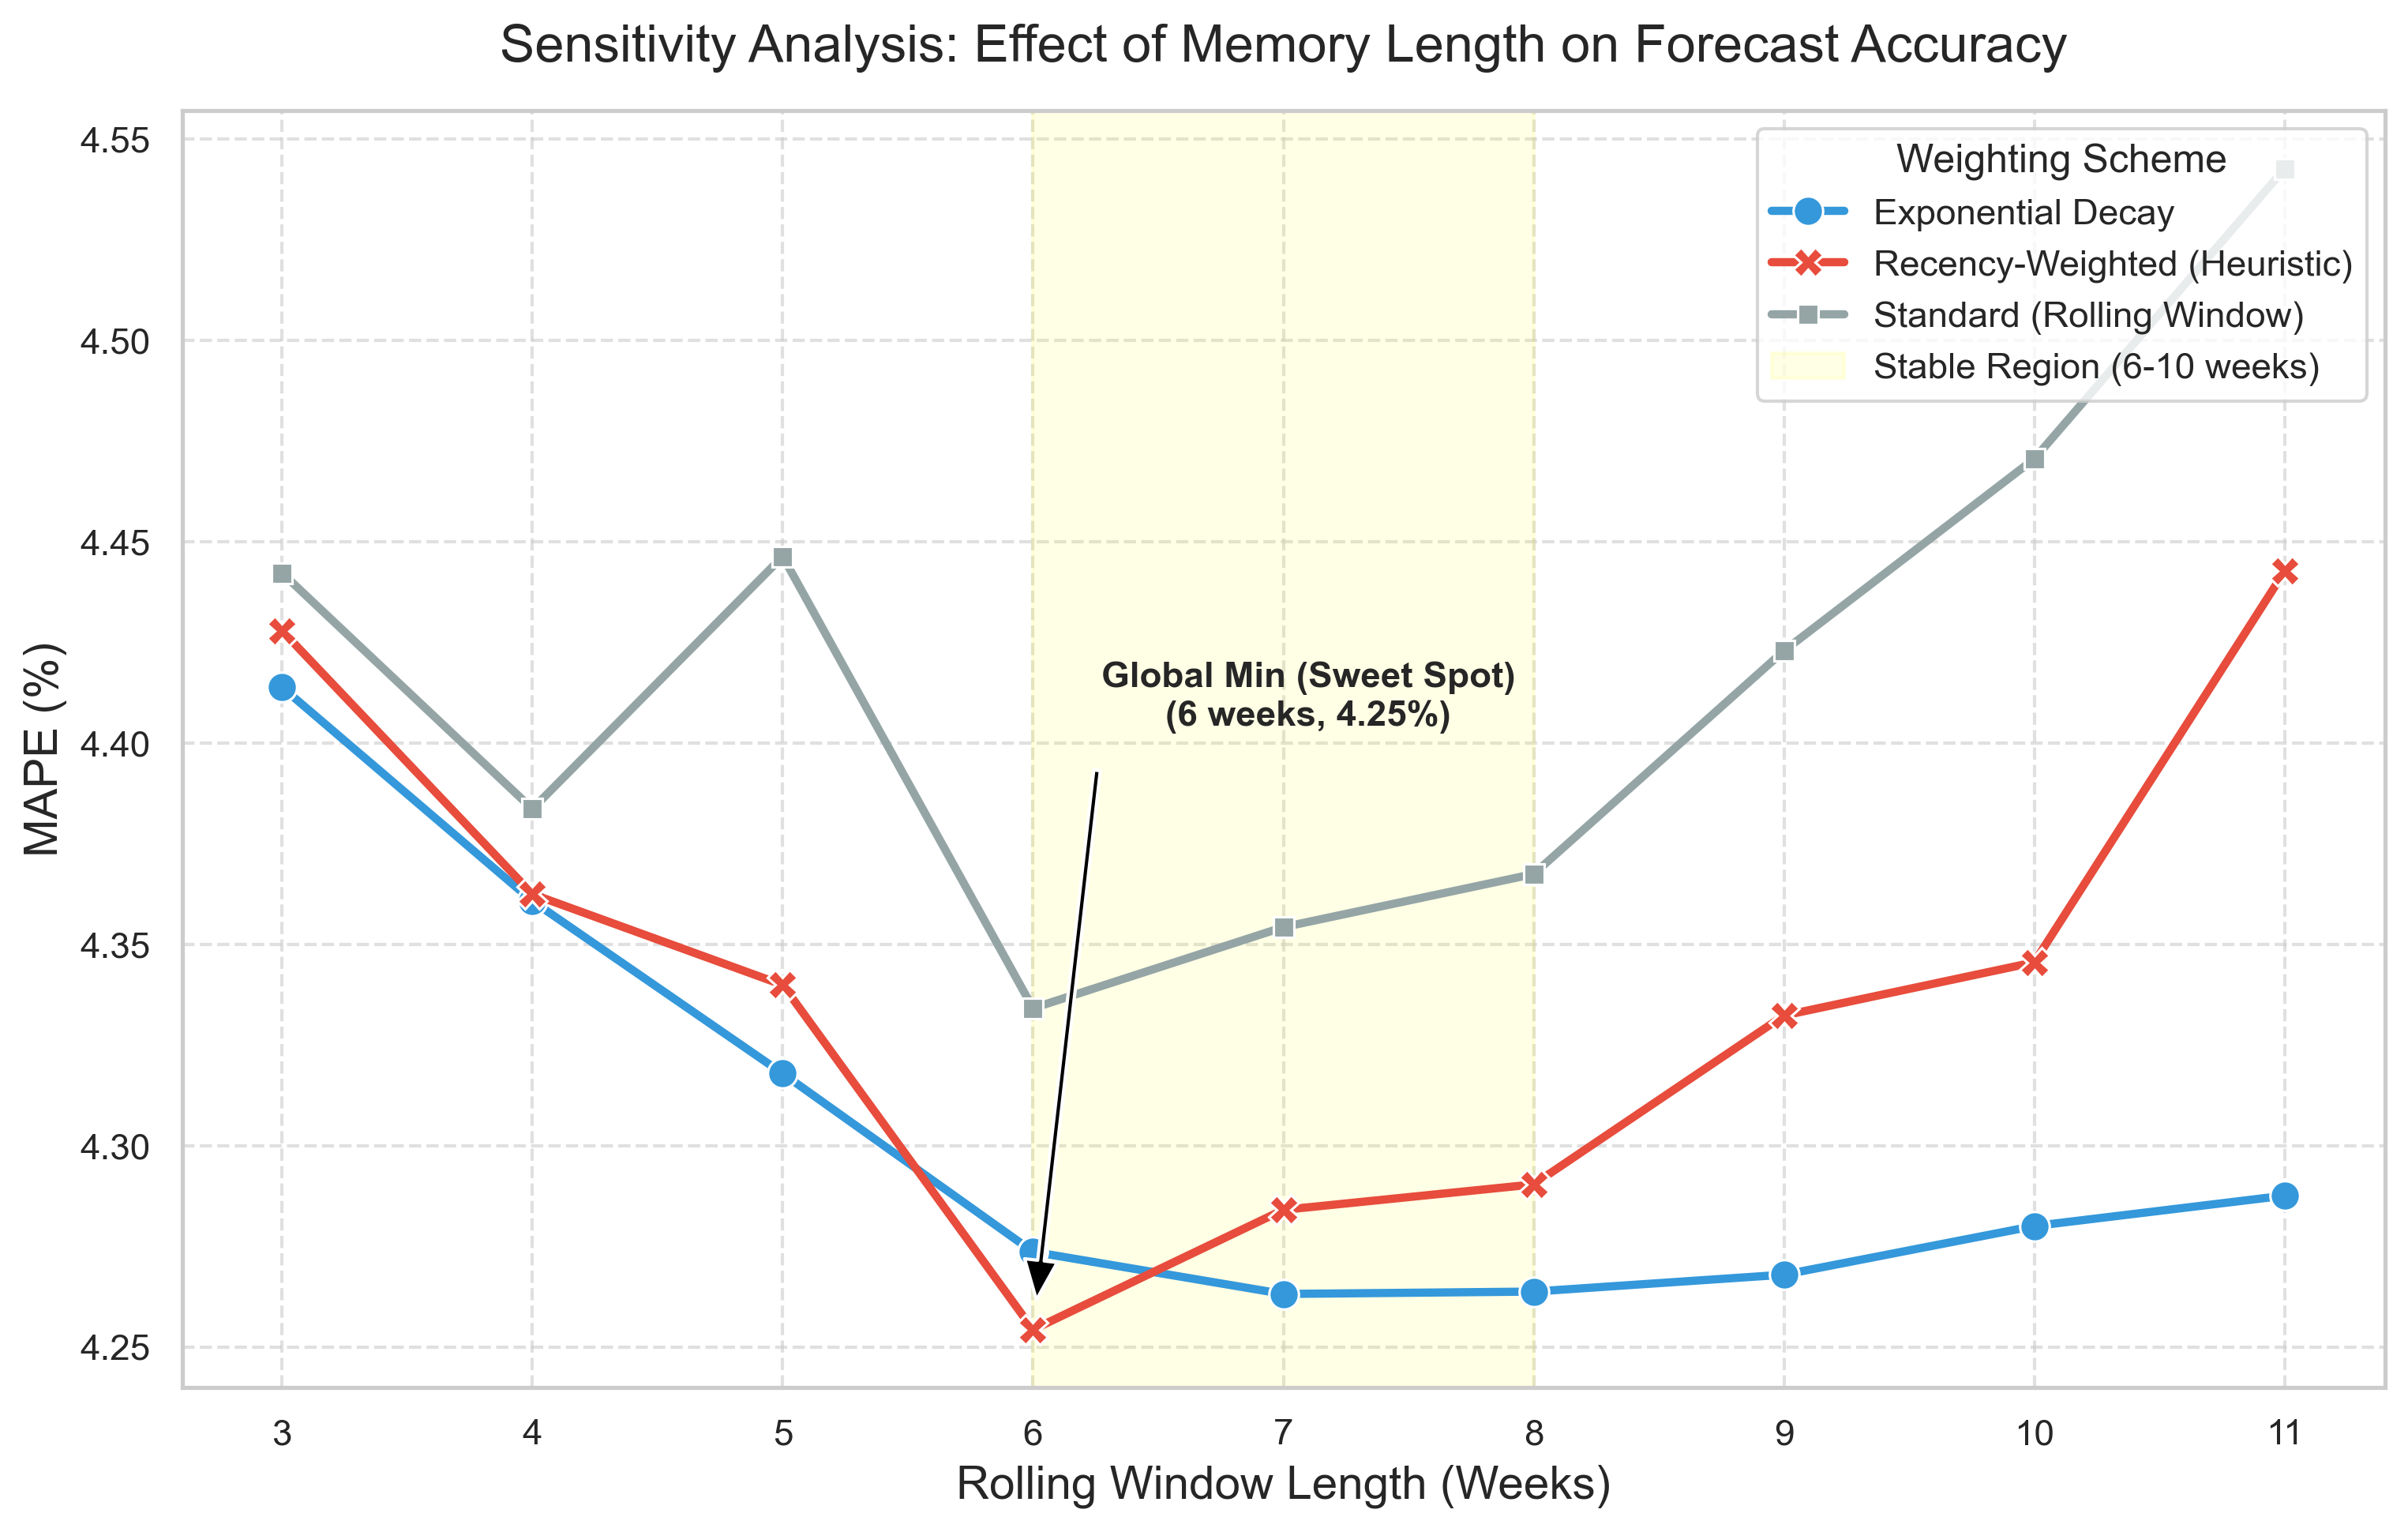
\includegraphics[width=0.8\textwidth]{sensitivity_analysis.png}
\caption{Sensitivity Analysis: Effect of Rolling Window Length on Forecast Accuracy (MAPE) using the Frank-Wolfe optimization. The analysis reveals a robust "sweet spot" around 6 weeks, balancing model stability with adaptability to recent trends.}
\label{fig:sensitivity}
\end{figure}

Figure \ref{fig:weights} illustrates the evolution of weights for the winning strategy. The system dynamically reallocates weights, effectively "hedging" against the failure of any single predictor.

\begin{figure}[H]
\centering
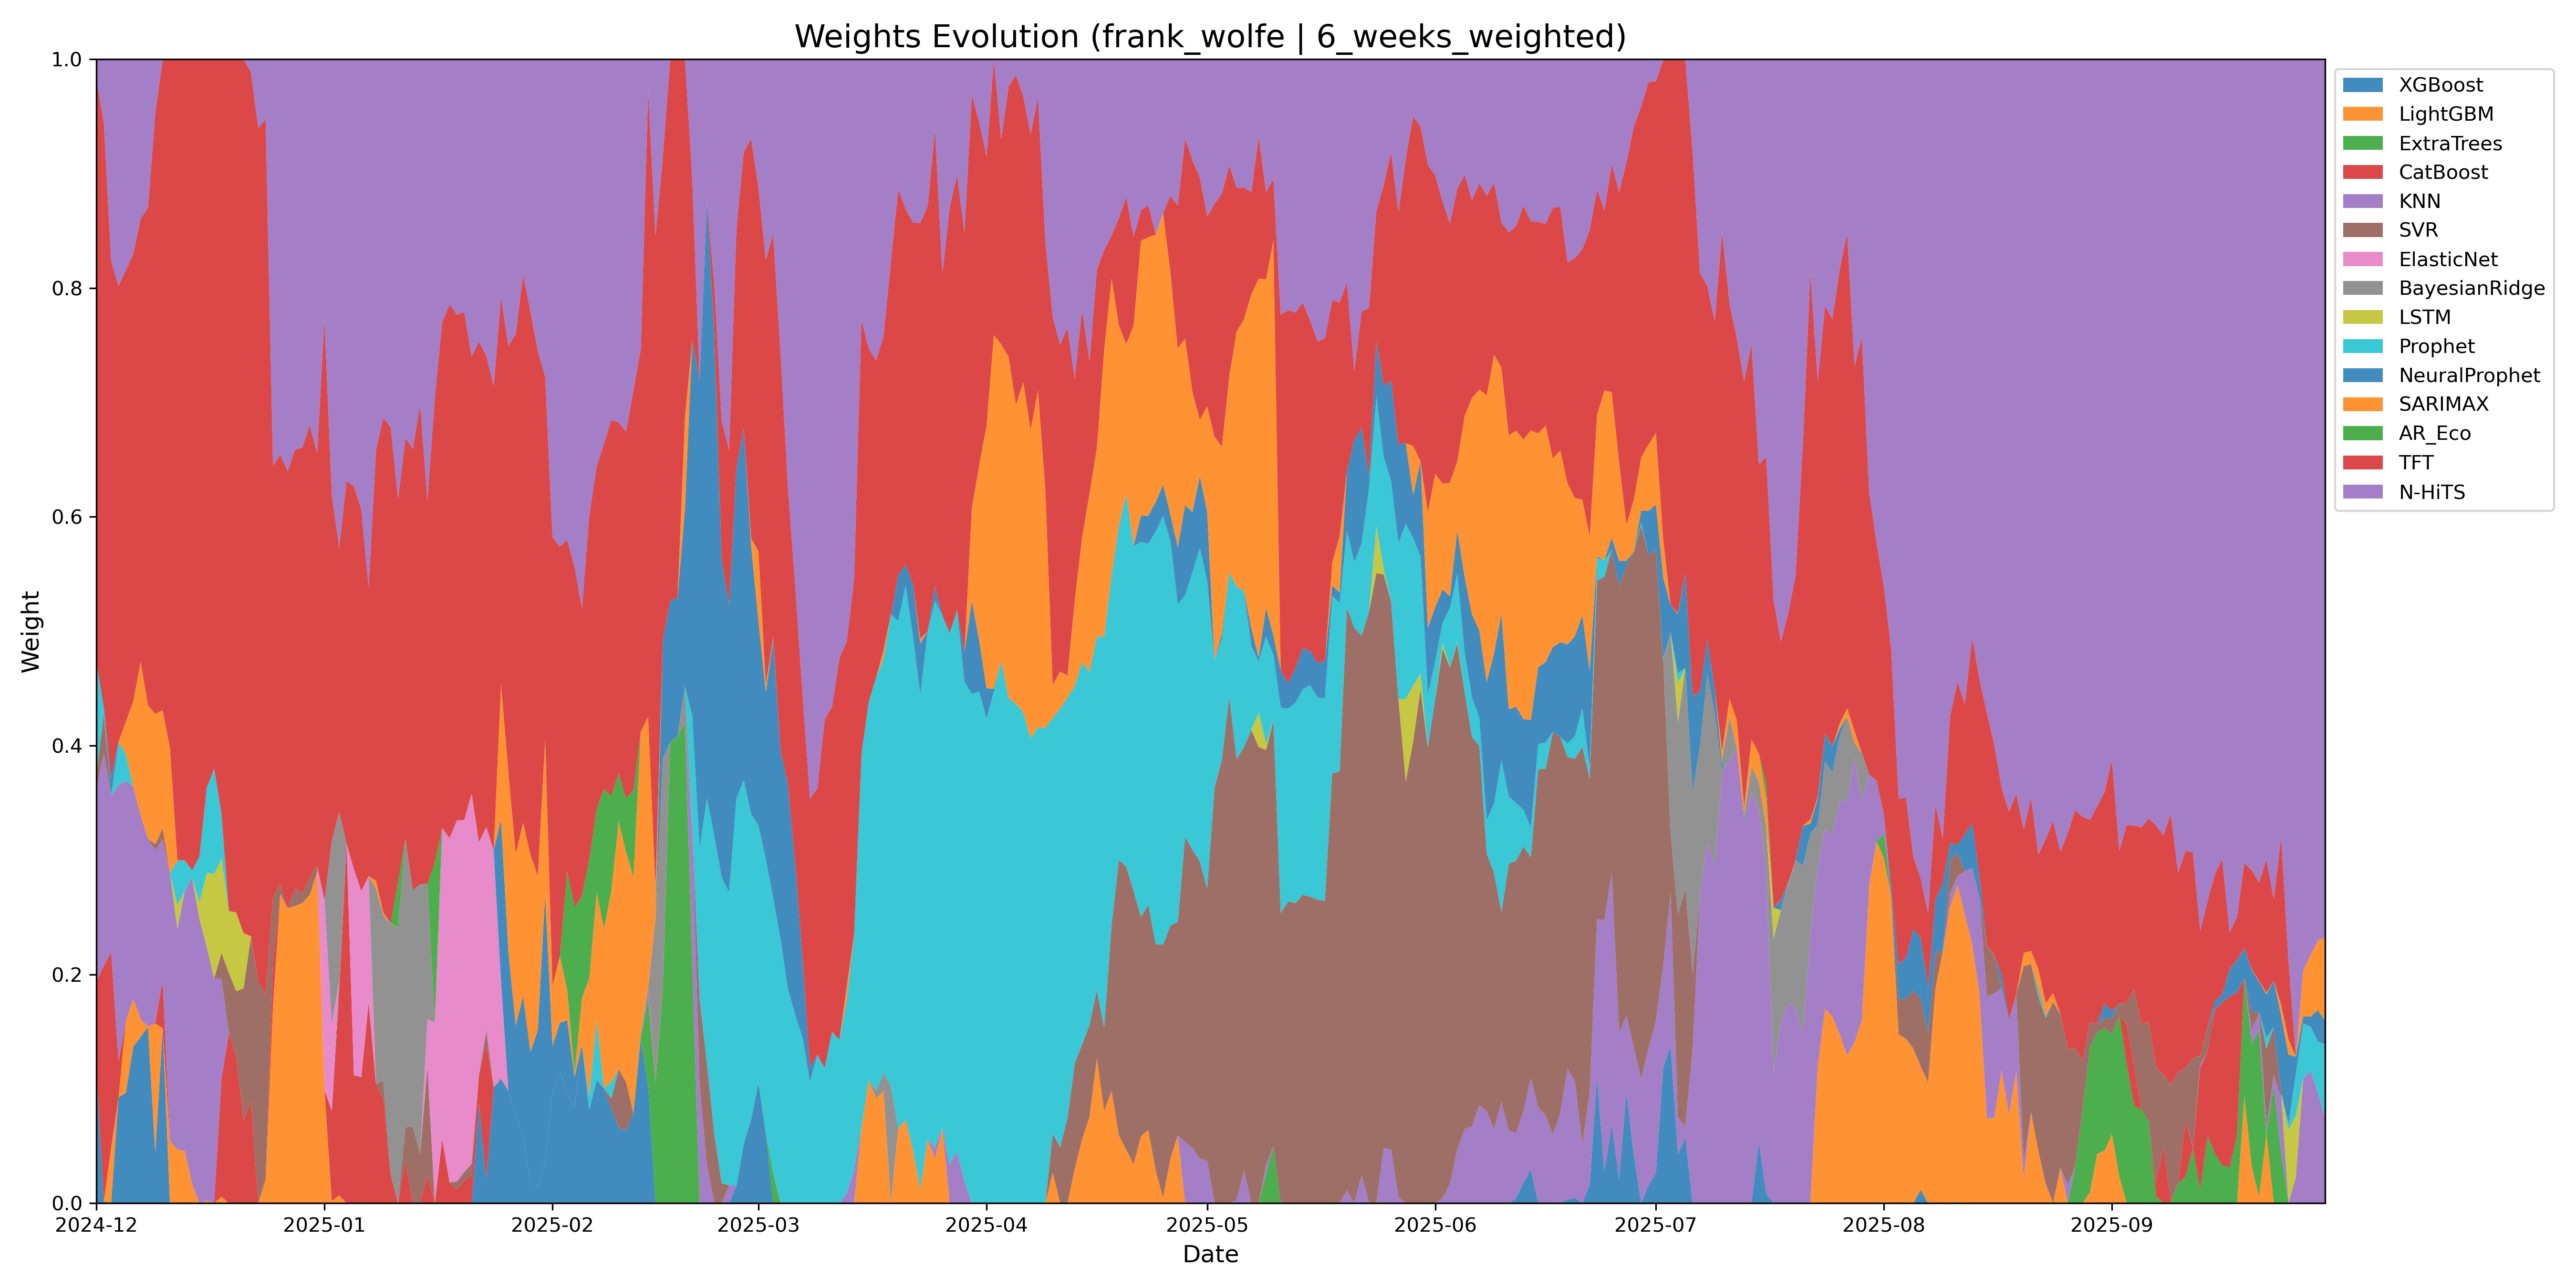
\includegraphics[width=0.95\textwidth]{weights_evolution_frank_wolfe_6_weeks_weighted.png}
\caption{Evolution of model weights over the test period (Frank-Wolfe, 6-week weighted window). The meta-learner actively adapts to changing market conditions by shifting weights between TFT, N-HiTS, and Gradient Boosting models.}
\label{fig:weights}
\end{figure}

%%%%%%%%%%%%%%%%%%%%%%%%%%%%%%%%%%%%%%%%%%
\section{Discussion}

The results confirm that the application of operations research methods to the weighting of machine learning predictions offers a transparent and controllable way to improve forecast accuracy. The 6-week weighted window appears to be a robust heuristic for the Czech gas market.

\textbf{Stability vs. Accuracy:} Although the difference in accuracy (0.01 p.p.) between \textbf{Frank-Wolfe} (MAPE 4.25\%) and \textbf{Ensemble Selection} (MAPE 4.26\%) is statistically negligible, we argue that Frank-Wolfe is the superior choice for production environments. Ensemble Selection is a discrete, greedy algorithm that selects models from a finite set of steps. This can lead to abrupt changes in weights ("bang-bang" behavior) when the underlying data shifts slightly. In contrast, Frank-Wolfe operates in a continuous space on the simplex, producing \textbf{smoother weight transitions} (as seen in Figure \ref{fig:weights}). For a market operator, this stability is crucial, as it mitigates the operational risk associated with abrupt day-to-day shifts in trading strategy. A Diebold-Mariano test further confirmed that the difference in accuracy between the two top strategies is not statistically significant ($p = 0.2669$), reinforcing the view that the selection should be driven by structural properties like stability rather than marginal performance gains.

\textbf{Interpretability:} Unlike black-box AutoML solutions, our Convex Weight Optimization framework maintains interpretability. The weights $\mathbf{w}$ directly represent the confidence in each underlying model (e.g., "today we trust N-HiTS 40\% and XGBoost 60\%"), effectively treating the forecast as an investment portfolio.

The poor performance of \textbf{Prophet} (MAPE 13.15\%) can be attributed to its additive nature and reliance on smooth Fourier terms for seasonality, which struggle to capture the sharp, non-linear demand spikes driven by sudden temperature drops in the Central European heating season.

%%%%%%%%%%%%%%%%%%%%%%%%%%%%%%%%%%%%%%%%%%
\section{Conclusions}

We presented a technical framework for optimizing gas consumption forecasts. By rigorously formulating the weighting problem and solving it via the Frank-Wolfe algorithm, we provide a scalable solution for daily energy operations. Our experiments show that this approach can reduce forecasting error (MAPE) to \textbf{4.25\%}, significantly outperforming both traditional statistical baselines and individual deep learning models. We also validated that a formally defined "Recency-Weighted" loss function ($\omega_t \in \{1, 3\}$) is as effective as more complex exponential weighing schemes.

%%%%%%%%%%%%%%%%%%%%%%%%%%%%%%%%%%%%%%%%%%
\vspace{6pt} 

%%%%%%%%%%%%%%%%%%%%%%%%%%%%%%%%%%%%%%%%%%
\authorcontributions{Conceptualization, J.J. and V.V.; methodology, V.V.; software, V.V.; validation, J.J. and V.V.; formal analysis, V.V.; writing---original draft preparation, V.V.; writing---review and editing, J.J. All authors have read and agreed to the published version of the manuscript.}

\funding{The author gratefully acknowledges support from the Internal Grant Agency, Faculty of Informatics and Statistics, Prague University of Economics and Business (Project No. F4/10/2024).}

%\institutionalreview{Not applicable.}

%\informedconsent{Not applicable.}

\dataavailability{Publicly available datasets were analyzed in this study. The data can be found at \url{https://www.ote-cr.cz/} and \url{https://open-meteo.com/en/docs/historical-weather-api}.} 

\acknowledgments{We thank the anonymous referees for their time and comments.}

\conflictsofinterest{The authors declare no conflict of interest.} 

%%%%%%%%%%%%%%%%%%%%%%%%%%%%%%%%%%%%%%%%%%
\begin{adjustwidth}{-\extralength}{0cm}
\reftitle{References}
\isAPAStyle{}{%
\begin{thebibliography}{999}

\bibitem[\protect\citeauthoryear{Boyd and Vandenberghe}{{2004}}]{ref_boyd}
Boyd, S., \& Vandenberghe, L. (2004). \textit{Convex Optimization}. Cambridge University Press.

\bibitem[\protect\citeauthoryear{Caruana et al.}{{2004}}]{ref_caruana}
Caruana, R., Niculescu-Mizil, A., Crew, G., \& Ksikes, A. (2004). Ensemble selection from libraries of models. In \textit{Proceedings of the 21st International Conference on Machine Learning} (p. 18). ACM.

\bibitem[\protect\citeauthoryear{Challu et al.}{{2023}}]{ref_nhits}
Challu, C., Olivares, K. G., Oreshkin, B. N., Ramirez, F. G., Canseco, M. M., \& Dubrawski, A. (2023). N-HiTS: Neural Hierarchical Interpolation for Time Series Forecasting. \textit{Proceedings of the AAAI Conference on Artificial Intelligence}, 37, 6989--6997.

\bibitem[\protect\citeauthoryear{Chen and Guestrin}{{2016}}]{ref_xgboost}
Chen, T., \& Guestrin, C. (2016). XGBoost: A Scalable Tree Boosting System. In \textit{Proceedings of the 22nd ACM SIGKDD International Conference on Knowledge Discovery and Data Mining} (pp. 785--794). ACM.

\bibitem[\protect\citeauthoryear{Dudek}{{2021}}]{Dudek2021}
Dudek, G. (2021). A Comprehensive Study of Random Forest for Short-Term Load Forecasting. \textit{Energies}, 14(21), 6922. 
%\url{https://doi.org/10.3390/en14216922}


\bibitem[\protect\citeauthoryear{Frank and Wolfe}{{1956}}]{ref_fw_orig}
Frank, M., \& Wolfe, P. (1956). An algorithm for quadratic programming. \textit{Naval Research Logistics Quarterly}, 3(1-2), 95--110.

\bibitem[\protect\citeauthoryear{Jaggi}{{2013}}]{ref_fw_jaggi}
Jaggi, M. (2013). Revisiting Frank-Wolfe: Projection-Free Sparse Convex Optimization. In \textit{Proceedings of the 30th International Conference on Machine Learning} (pp. 427--435). PMLR.

\bibitem[\protect\citeauthoryear{Ke et al.}{{2017}}]{ref_lgbm}
Ke, G., Meng, Q., Finley, T., Wang, T., Chen, W., Ma, W., Ye, Q., \& Liu, T.-Y. (2017). LightGBM: A Highly Efficient Gradient Boosting Decision Tree. \textit{Advances in Neural Information Processing Systems}, 30.

\bibitem[\protect\citeauthoryear{Lim et al.}{{2021}}]{ref_tft}
Lim, B., Arik, S. O., Loeff, N., \& Pfister, T. (2021). Temporal Fusion Transformers for Interpretable Multi-horizon Time Series Forecasting. \textit{International Journal of Forecasting}, 37(4), 1748--1764.

\bibitem[\protect\citeauthoryear{Nalcaci et al.}{{2019}}]{ref_mdpi_energies_1}
Nalcaci, G., Ozmen, A., \& Weber, G. W. (2019). Long-term natural gas consumption forecasting with MARS and CMARS models. \textit{Energies}, 12(10), 1989.

\bibitem[\protect\citeauthoryear{Oliveira and Torgo}{{2014}}]{ref_oliveira}
Oliveira, M., \& Torgo, L. (2014). Ensembles for Time Series Forecasting. \textit{Proceedings of the Asian Conference on Machine Learning}, 39, 360--370.

\bibitem[\protect\citeauthoryear{OTE}{{2025}}]{ref_ote}
OTE, a.s. (2025). \textit{Metodika teplotního přepočtu TDD pro rok 2023}. Available online: \url{https://www.ote-cr.cz/} (accessed on 12 December 2025).

\bibitem[\protect\citeauthoryear{Paszke et al.}{{2019}}]{ref_pytorch}
Paszke, A., Gross, S., Massa, F., Lerer, A., Bradbury, J., Chanan, G., Killeen, T., Lin, Z., Gimelshein, N., Antiga, L., et al. (2019). PyTorch: An Imperative Style, High-Performance Deep Learning Library. \textit{Advances in Neural Information Processing Systems}, 32.

\bibitem[\protect\citeauthoryear{Pedregosa et al.}{{2011}}]{ref_scikit}
Pedregosa, F., Varoquaux, G., Gramfort, A., Michel, V., Thirion, B., Grisel, O., Blondel, M., Prettenhofer, P., Weiss, R., Dubourg, V., et al. (2011). Scikit-learn: Machine Learning in Python. \textit{Journal of Machine Learning Research}, 12, 2825--2830.

\bibitem[\protect\citeauthoryear{Prokhorenkova et al.}{{2018}}]{ref_catboost}
Prokhorenkova, L., Gusev, G., Vorobev, A., Dorogush, A. V., \& Gulin, A. (2018). CatBoost: Unbiased Boosting with Categorical Features. \textit{Advances in Neural Information Processing Systems}, 31.

\bibitem[\protect\citeauthoryear{Taylor and Letham}{{2018}}]{ref_prophet}
Taylor, S. J., \& Letham, B. (2018). Forecasting at Scale. \textit{The American Statistician}, 72(1), 37--45.

\bibitem[\protect\citeauthoryear{Wang et al.}{{2020}}]{ref_mdpi_math_1}
Wang, J., Du, Y., \& Wang, J. (2020). LSTM based long-term energy consumption forecasting with periodicity. \textit{Mathematics}, 8(12), 2139.

\bibitem[\protect\citeauthoryear{Wu and Levinson}{{2021}}]{ref_wu_review}
Wu, H., \& Levinson, D. (2021). The Ensemble Approach to Forecasting: A Review and Synthesis. \textit{Transportation Research Part C: Emerging Technologies}, 132, 103357.

\bibitem[\protect\citeauthoryear{Zhang et al.}{{2022}}]{ref_mdpi_energies_2}
Zhang, Y., Li, J., \& Li, X. (2022). Ensemble forecasting of natural gas consumption using dynamic weighting. \textit{Energies}, 15(3), 882.

\bibitem[\protect\citeauthoryear{Zippenfenig}{{2023}}]{ref_openmeteo}
Zippenfenig, P. (2023). Open-Meteo.com Weather API [Computer software]. Zenodo. \url{https://doi.org/10.5281/ZENODO.7970649}

\end{thebibliography}
}
\PublishersNote{}
\end{adjustwidth}

%%%%%%%%%%%%%%%%%%%%%%%%%%%%%%%%%%%%%%%%%%

\end{document}